\documentclass{article}
\setlength{\parskip}{5pt} % esp. entre parrafos
\setlength{\parindent}{0pt} % esp. al inicio de un parrafo
\usepackage{amsmath} % mates
\usepackage[sort&compress,numbers]{natbib} % referencias
\usepackage{url} % que las URLs se vean lindos
\usepackage[top=25mm,left=20mm,right=20mm,bottom=25mm]{geometry} % margenes
\usepackage{hyperref} % ligas de URLs
\usepackage{graphicx} % poner figuras
\usepackage[spanish]{babel} % otros idiomas
\usepackage[utf8]{inputenc}
\author{Jesus Alberto Funes Mendoza  \\
Melissa Lizeth Galindo Reyes  \\
Ramón Samuel Blanco Ramirez  \\
Aída Mata Moreno  \\
Miriam Itzel Mata Porras  \\ 
Víctor Adrián Higuera Vázquez} % author
\title{Actividad 4: La biomecánica de la mano} % titulo
\date{\today}
\usepackage{float} 
\begin{document} % inicia contenido

\maketitle % cabecera

\begin{abstract} % resumen

\end{abstract}

\section{Introducción}\label{intro} % seccion y etiqueta
En este tema que es la biomecánica de la mano, nos ayudará a conocer como cada uno tiene su función, en un los seres humanos sabes el cómo funciona, pero realmente no conocemos muy a fondo para que sirve cada dedo, que tanta fuerza se necesita para tomar un lápiz y hasta con que dedo es con el que sujetamos, pero cuando se utiliza una prótesis, se tiene que conocer y verificar la fuerza, para que la persona lo pueda utilizar, así mismo es importante también conocer las funciones de cada dedo y también van e las mano las articulaciones ya que es una gran parte clave ya que esta nos da el tipo de movimiento debemos de tener.

\section{Desarrollo}
Desde la pinza del crustáceo hasta la mano del simio realizan una oposición, ninguna puede conseguirla con la sutileza y precisión de la mano humana.

\subsection{Eje de los dedos}
Se denomina como la línea imaginaria por la cual podemos estudiar los movimientos de las articulaciones, como primer movimiento esta el de la figura A que el estado natural donde vemos que los ejes del dedo índice y pulgar cruzan con el eje del dedo medio mientras que el dedo meñique y anular son divergentes, al separar los dedos como en la figura B todos los ejes convergen entre si, al juntarlos como en la figura C puede llegar a parecer que son ejes paralelos pero convergen en un punto mas lejano debido a que los dedos son mas anchos de la base que de la punta y al hacer un puño como en la imagen D todos los ejes convergen en el punto llamado talón de la mano
\begin{figure}[H]
    \centering
    %Modificando los parámetros de height puedes cambiar el tamaño de tu imagen.
    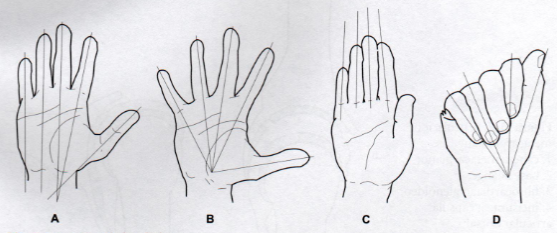
\includegraphics[height=7cm]{Imagenes/1.png}
    \caption{\textit{Lineas imaginarias de los movimientos de las articulaciones de la mano.}} %Nombre de la figura
    \label{exemploLabel}
    \end{figure}

\subsection{Articulaciones}
\textbf{Metacarpofalángicas:} Son del tipo condíleo, y permiten por tanto movimientos activos o flexoextensión, palmar y dorsal, abducción, abducción y pequeños movimientos pasivos de rotación axial.
Se conforma por: 

1.	Cabeza metacarpiano.

2.	Base falange.

3.	Fibrocartílago glenoideo.

4.	Incisura.

5.	Cápsula articular dorsal.

6.	Cápsula articular palmar.

\begin{figure}[H]
    \centering
    %Modificando los parámetros de height puedes cambiar el tamaño de tu imagen.
    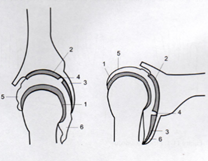
\includegraphics[height=7cm]{Imagenes/2.png}
    \caption{\textit{Ubicaciones de las metacarpofalángicas}} %Nombre de la figura
    \label{exemploLabel}
    \end{figure}
    
\textbf{Interfalángicas:} Las articulaciones interfalángicas son del tipo troclear, y permiten sólo un tipo de movimiento que es el de flexoextensión. Al igual que las articulaciones metacarpofalángicas, la superficie articular que presenta la cabeza de la primera falange es mucho mayor que la de la base de la segunda falange por lo que las mismas razones biomecánicas, en la base de la segunda falange existe un fibrocartílago glenoide que en el momento de la flexión se desliza sobre la cara palmar de la falange proximal. EC: extensor común; FCS: flexor común superficial; FCP: flexor común profundo; LM: lengüeta meda; LL: lengüetas laterales.
\begin{figure}[H]
    \centering
    %Modificando los parámetros de height puedes cambiar el tamaño de tu imagen.
    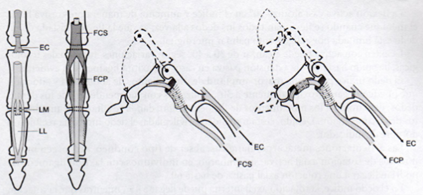
\includegraphics[height=7cm]{Imagenes/3.png}
    \caption{\textit{}} %Nombre de la figura
    \label{exemploLabel}
    \end{figure}

\textbf{Trapeciometacarpiana:} Se trata de una articulación básica dentro de la biomecánica del pulgar, integra la llamada columna osteoarticular de éste, compuesta por el escafoides, trapecio, primer metacarpiano y primera y segunda falanges.

\textbf{Metacarpo falángica del pulgar:} Articulación del tipo condíleo que permiten teoría 2 movimientos, pero realmente realiza también movimientos de rotación axial tanto activos como pasivos, lo que confiere una gran importancia ya que estos movimientos no son habituales en las articulaciones de estas características.

\textbf{Interfalángica del pulgar:} Es de tipo troclear como el resto de las articulaciones interfalángicas y permite solo movimientos de flexoextensión.

\subsection{Tendones}
\textbf{Flexores:} El flexor común profundo de los dedos inserten la base de la tercera falange, después de perforar el flexor común superficial que se divide en 2 lengüetas de la articulación metacarpofalángicas para insertarse distalmente en las caras laterales de la segunda falange. Los tendones flexores están envueltos por una vaina cilíndrica que contiene un líquido sinovial que actúa como lubricante para evitar o disminuir la fricción en los movimientos del tendón contra las prominencias óseas en los puntos de la angulación de las articulaciones.

\textbf{Extensores:} Los músculos de los tendones extensores de los dedos nacen en el epicóndilo humeral y se dirigen hacia la cara dorsal. Son músculos extrínsecos que transcurren por correderas a nivel de la muñeca y por debajo del ligamento anular superior del carpo. 

\subsection{Acción de los musculos interoseos y lubricales}
Son fundamentales para realizar los movimientos de lateralidad y flexoextensión de los dedos.

\textbf{Acción del extensor común:} el extensor común de los dedos es extensor de la primera falange y solo actúa sobre la segunda y tercera, cuando la muñeca y las articulaciones metacarpofalángicas están en flexión.

\textbf{Acción de músculos interóseos:} los músculos interóseos son flexores de la primera falange y extensores de la segunda y tercera dependiendo del grado de flexión de las articulaciones metacarpo falángicas y de la tensión de la extensión común de los dedos.

\textbf{Acción de los músculos lumbricales:} estos pequeños músculos intrínsecos de la mano desempeñan un papel esencial en los movimientos de flexoextensión de los dedos, ya que al estar situados en un plano más palmar que el ligamento transverso intermetacarpiano, tiene ángulos de incidencia de 35° con respecto a la primera falange, lo que les permite flexionarla, aunque ésta se encuentra en hiperextensión.

\subsection{Oposición del pulgar}
La oposición del pulgar resulta de la coordinación de varios movimientos como son la ante pulsión y abducción del primer metacarpiano, junto con la rotación axial del primer metacarpiano y de la primera falange. Gracias a este movimiento de rotación axial, el dedo pulgar partiendo de una posición inicial en extensión máxima, con la palma muy abierta se coloca en una posición intermedia frente al dedo índice y termina en una oposición máxima contactando con el dedo meñique.

\subsection{Funciones de la mano}
La mano tiene múltiples Funciones siendo la más importante la de tocar que es una función sensitiva y la depresión que es una función motora.

La posición de los elementos móviles de la mano para asistir los objetos y adaptarse a su forma presente numerosas combinaciones.
\begin{figure}[H]
    \centering
    %Modificando los parámetros de height puedes cambiar el tamaño de tu imagen.
    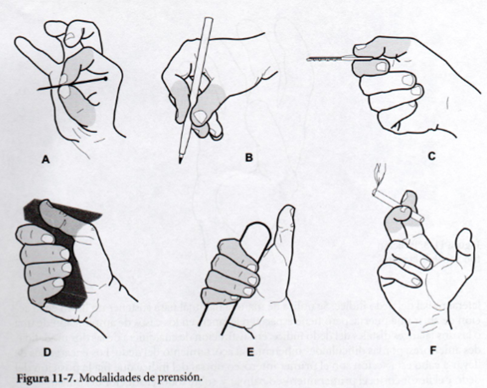
\includegraphics[height=7cm]{Imagenes/4.png}
    \caption{\textit{Acciones y posiciones que puede realizar la mano.}} %Nombre de la figura
    \label{exemploLabel}
    \end{figure}


\section{Conclusiones}
En esta actividad nos ayudó a conocer más sobre la mano biomecánica, cumplimos con nuestro objetivo, ya que ampliamos más nuestro conocimiento en este tema, si bien es un tema extenso, ya que la mano tiene diferentes movimientos y más el conocer el movimiento de los dedos, por que cada uno tiene diferentes funciones, los cuales se complementan entre sí, es importante el conocer bien sus movimientos, ya que si se hace una prótesis y no se conoce muy a fondo  esta prótesis quedaría mal hecha y hasta podría dañar a un paciente, este pdf nos ayudó mucho a unir más nuestros conocimientos y el cómo ayudarnos.

\bibliography{bib}
\bibliographystyle{plainnat}
\end{document}

